\chapter{Analýza a návrh}

Tato kapitola popisuje proces analýzy požadavků a návrhu systému.
V první části jsou popsány metody použité při analýze požadavků. V druhé části jsou popsány návrhy systému, které byly vytvořeny na základě analýzy požadavků.
Analýza je nezávislá na technologiích použitých při následné implementaci.

\section{Analýza požadavků}

Analýza požadavků je proces, který má za cíl získat informace o požadavcích na systém. Na základě průběžných konzultací s vedoucím práce, Ing. Markem Jílkem, a 
Bc. Lucií Annou Procházkovou, členy týmu organizátorů akce SummerJob, byly získány podrobné informace o procesu organizace akcí a požadované funkcionalitě nové aplikace.
Tyto konzultace byly prováděny i dále během vývoje systému, aby bylo zajištěno, že systém bude plnit požadavky organizátorů akce. Pomocí této agilní metody
bylo možné průběžně reagovat na případné změny a seznamovat budoucí uživatele s aktuálním stavem systému.

V této práci bude kromě obecných pojmů pro jednotlivé součásti systému použita také existující terminologie z akce SummerJob: \textit{pracant} je označení pro brigádníka, \textit{job} je označení pro práci, kterou brigádník vykonává.

\subsection{Funkční požadavky}
\label{sec:functional-requirements}

Funkční požadavky popisují funkcionalitu požadované aplikace, specifikují možnosti, vlastnosti a operace, které musí být možné provádět.
Jsou základem při návrhu a implementaci systému.

\begin{itemize}
    \item \textbf{FP1. Přihlášení a registrace:} uživatelé systému musí být schopni se přihlásit do systému, pokud jsou registrováni v právě probíhajícím ročníku. Registraci není třeba implementovat, probíhá externě a schvalují ji organizátoři akce.
    \item \textbf{FP2. Správa oprávnění a uživatelských účtů:} uživatelé systému mají různá oprávnění, která určují, co všechno mohou v systému provádět. Oprávnění jsou rozdělena podle přístupu ke správě jednotlivých položek (pracanti, joby, auta, plánování). Administrátor má možnost nastavit oprávnění jednotlivým uživatelům, případně uživateli zcela zakázat přístup do systému.
    \item \textbf{FP3. Správa pracantů:} organizátoři akce musí být schopni spravovat seznam pracantů. Musí být možné přidávat, mazat a upravovat informace o pracantech. Tyto informace zahrnují jméno a příjmení, e-mail, telefonní číslo, alergie, dostupnost pracanta v jednotlivých dnech akce, informaci, zda a kdy se chce pracant účastnit adorací. Organizátoři sami během akce pracují a patří tedy mezi pracanty.
    \item \textbf{FP4. Správa jobů:} organizátoři akce musí být schopni spravovat seznam jobů. Musí být možné přidávat, mazat a upravovat informace o jobech. Tyto informace zahrnují název jobu, popis jobu, lokalitu, kontaktní osobu, alergeny na místě, celkový počet pracantů, které je možné přiřadit k jobu, požadovaný počet silných pracantů a počet dní nutných na splnění práce. U prací je evidována dostupnost občerstvení a sprchy. Jednotlivé joby musí být možné označit jako splněné, případně prioritní. Prioritní joby musí být v seznamu jobů odlišeny od ostatních a slouží ke zvýšení viditelnosti prací, které jsou pro organizátory důležité. V jobech musí být možné vyhledávat.
    \item \textbf{FP5. Správa aut:} organizátoři mohou spravovat dostupná auta. U aut se eviduje počet míst, vlastník (pracant) a najeté kilometry. Na základě najetých kilometrů během akce se po skončení akce počítá kompenzace pro řidiče. Systém by měl umožnit evidenci, zda byla kompenzace vyplacena.
    \item \textbf{FP6. Správa plánů:} zodpovědné osoby mohou tvořit plány na jednotlivé dny, přidávat joby do plánů, přidávat pracanty do jobů, plánovat dopravu pro jednotlivé joby. Pracanti z různých jobů mohou sdílet dopravu. Systém musí podporovat současnou práci více uživatelů během tvorby plánu. Plány musí být možné zobrazit v tisknutelném formátu.
    \item \textbf{FP7. Automatický plánovač:} systém musí být schopný na žádost oprávněného uživatele naplánovat rozvrh pracantů na zadané joby. Po přidání jobů do plánu a vyžádání vygenerování plánu plánovač přiřadí pracanty na joby a naplánuje dopravu. Přitom respektuje dostupnost pracantů v daný den, alergie, požadovaný počet silných pracantů na jobu a požadavky na adoraci.
    \item \textbf{FP8. Správa ročníků:} systém musí být schopný spravovat více ročníků akce SummerJob. Administrátor systému má možnost přepínat mezi jednotlivými ročníky. Každý ročník má název a časové rozpětí.
    \item \textbf{FP9. Správa oblastí:} systém musí být schopný spravovat oblasti, do kterých jsou joby rozděleny. U oblasti se eviduje nutnost dopravy autem a možnost adorace. Oblasti jsou vztaženy k aktuálnímu ročníku.
    \item \textbf{FP10. Záznam systémových změn:} systém musí být schopný zaznamenávat změny, které uživatelé provádějí. Záznamy musí obsahovat časové razítko, uživatele, který změnu provedl a popis změny. Administrátor má možnost zobrazit záznamy změn.
    \item \textbf{FP11. API:} systém poskytuje API, které umožňuje přístup k datům systému. API musí umožňovat provádět operace na úrovni srovnatelné s webovou aplikací.
\end{itemize}

\subsection{Nefunkční požadavky}
\label{sec:nonfunctional-requirements}

Nefunkční požadavky se týkají výkonu, spolehlivosti, bezpečnosti, škálovatelnosti a dalších aspektů systému. Nepopisují funkce systému, ale zaměřují se na celkovou kvalitu, provozuschopnost a výkonnost.

\begin{itemize}
    \item \textbf{NP1. Bezpečnost:} systém bude využívat přihlášení a ověření práv uživatelů pro přístup k datům. Uživatel bez potřebného oprávnění nesmí mít přístup datům, pro které je dané oprávnění nezbytné. Výjimkou je přístup k datům potřebným pro vykonávání činností, na které má uživatel oprávnění, například přístup ke jménům pracantů při přidávání nového auta do systému za účelem určení majitele. Přístup k databázi nebude možný přímo z internetu, ale pouze přes webovou aplikaci nebo API. Spojení mezi uživatelem a aplikací musí být šifrované.
    \item \textbf{NP2. Udržovatelnost a rozšiřitelnost:} výsledná aplikace využívá rozšířené technologie a standardy, které umožňují další rozšíření. K dispozici je dokumentace popisující fungování aplikace a použité technologie. Vývojáři systému mají možnost snadno rozšiřovat aplikaci o nové funkce.
    \item \textbf{NP3. Nezávislost na platformě:} aplikace nesmí být vázána na konkrétní operační systém. Vývojáři systému mají možnost snadno přenést aplikaci na jinou platformu. Webová aplikace musí být responzivní a použitelná na současných mobilních zařízeních i počítačích.
    \item \textbf{NP4. Rychlost plánovače:} plánovač musí být schopen vygenerovat plán pro 150 pracantů a 50 jobů do 15 sekund.
\end{itemize}

\section{Návrh systému}

V této kapitole je popsán návrh systému na základě provedené analýzy. Návrh popisuje celkovou architekturu systému, webovou aplikaci a API, databázi a plánovací systém.
Systém bude současně obsluhovat jednotky až desítky uživatelů, není tedy nutné řešit škálovatelnost. Vzhledem k povaze akce SummerJob, která zajišťuje práci
v malých vesnicích a obcích v jedné oblasti, není možné, že budou systém využívat stovky či tisíce uživatelů současně.

\subsection{Architektura systému}

Aby bylo možné k vytvořenému systému přistupovat z libovolného zařízení, bude uživatelské rozhraní implementováno jako responzivní webová aplikace. Serverová část 
bude poskytovat API pro přístup k datům uloženým v databázi. Automatický plánovač bude vyčleněn do samostatné služby, aby bylo možné v případě potřeby provádět
jeho aktualizaci bez nutnosti zásahu do webového serveru. Toto řešení umožní v případě nutnosti optimalizace vybrat libovolný jazyk a technologie pro implementaci plánovače.
Aby nedošlo k selhání komunikace mezi serverovou částí webové aplikace a plánovačem v případě dočasného výpadku plánovače nebo jeho nedostupnosti při plánování, bude komunikace
mezi těmito komponentami probíhat pomocí fronty zpráv. Komunikace mezi jednotlivými komponentami bude probíhat pomocí standardních protokolů a rozhraní, aby bylo možné
části nahradit jinými, pokud vybrané komponenty nebudou vyhovovat.
Schéma architektury systému je na obrázku \ref{fig:architecture}.

\begin{figure}[h]
    \centering
    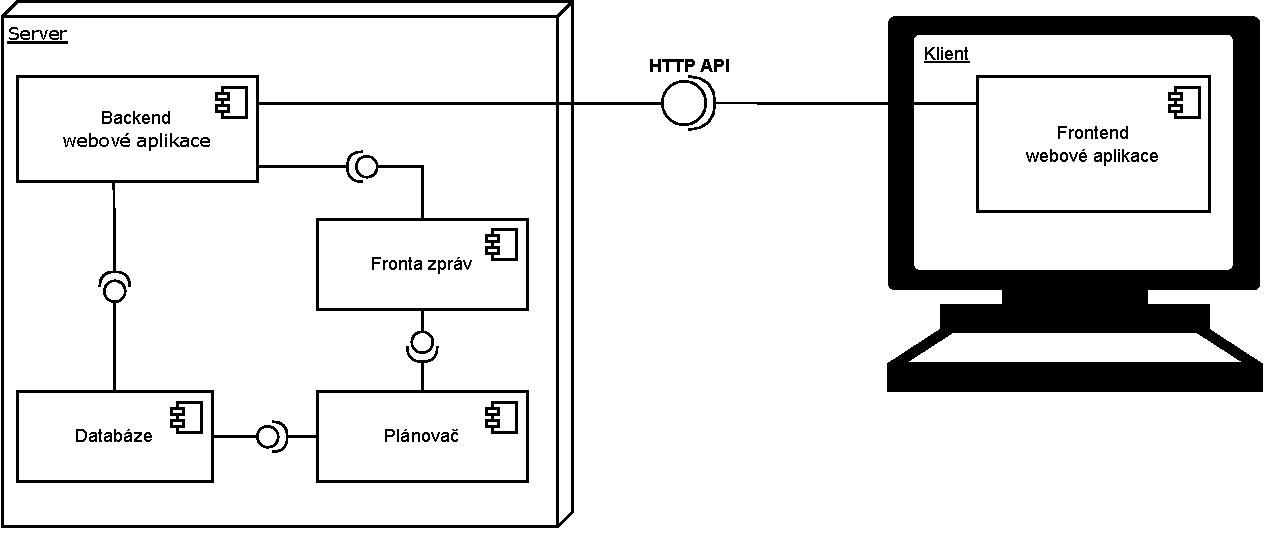
\includegraphics[width=\textwidth]{chapters/images/architektura}
    \caption{Architektura systému}
    \label{fig:architecture}
\end{figure}

\subsection{Webová aplikace a API}

Webová aplikace bude hlavním uživatelským rozhraním pro přístup k datům systému. Organizátoři budou přes webové rozhraní evidovat všechny potřebné údaje, vytvářet plány,
spravovat uživatelské účty, spouštět automatický plánovač a tisknout plány. K webové aplikaci budou účastníci i organizátoři přistupovat i přes mobilní zařízení během akce, 
je tedy nezbytné, aby byla aplikace responzivní. Serverová a klientská část webové aplikace budou splňovat všechny funkční požadavky, které jsou popsány v kapitole \ref{sec:functional-requirements}.
Funkční požadavek 11 dále určuje, že systém musí poskytovat API, které umožňuje přístup k datům systému. Aby bylo zajištěno,
že API poskytuje funkcionalitu shodnou s funkcionalitou webové aplikace, bude webová aplikace komunikovat se serverovou částí přes API.

Pro implementaci klientské části je vhodné využít moderní, udržované a dobře zdokumentované technologie. Akce SummerJob se často konají v pohraničních oblastech,
kde je možné, že uživatelé budou mít problémy s přístupem k internetu. Zvolené technologie musí umožňovat zotavení z chyb v případě nepodařených požadavků na server
a celkové množství přenesených dat by mělo být co nejmenší.

Přihlašování do webové aplikace je možné provést pomocí uživatelského jména a hesla, pomocí přihlašovacího odkazu nebo přes poskytovatele identity třetí strany.
Přihlašování pomocí uživatelského jména a hesla představuje největší bezpečnostní riziko, protože uživatelé mohou používat stejné heslo pro více služeb. Bylo by nutné
zajistit korektní správu hesel, jejich bezpečné ukládání a kontrolu. Dále by bylo nutné implementovat funkce pro obnovu hesla v případě zapomenutí.

Mezi poskytovatele identit patří například Google, Facebook nebo GitHub. Přihlašování přes poskytovatele třetí strany je výhodné pro uživatele, protože nemusí vytvářet
nový účet pro tuto aplikaci. Také nebude nutné v aplikaci zajišťovat správu a životní cyklus hesel. Tento způsob přihlašování však není vhodný pro uživatele,
kteří služby těchto poskytovatelů nevyužívají.

Přihlašování pomocí přihlašovacího odkazu zaslaného na e-mailovou adresu je vhodné pro uživatele, kteří nechtějí vytvářet nový účet a nechtějí používat služby poskytovatelů třetí strany.
V aplikaci nebude nutné implementovat funkce pro správu hesel, ale bude nutné implementovat funkce pro odesílání e-mailů. Všichni uživatelé musí při registraci na akci
vyplnit e-mailovou adresu, takže tato funkce bude dostupná pro všechny účastníky. Jedná se o preferované řešení. Pro implementaci této funkcionality může být využita
externí knihovna.

Aplikace slouží primárně pro organizátory akce. Volitelně je možné povolit přístup brigádníkům, kteří si v aplikaci mohou prohlížet přiřazenou práci na aktuální den a nastavit osobní údaje.
Pokud bude tato funkcionalita implementována, bude možné při dalším vývoji zpřístupnit pracovníkům další informace, např. nástěnku s informacemi.

\subsection{Databáze}

Databáze bude sloužit jako hlavní úložiště dat systému pro všechny potřebné údaje. Jedná se převážně o seznamy uživatelů, prací, aut, plánů a vazby mezi nimi.
Databáze bude uchovávat data o rozsahu několika stovek záznamů pro každý ročník. Běžné databázové systémy jsou schopny zpracovat takové množství dat, a tak není potřeba
klást na výběr databáze žádné specifické požadavky.

Na základě požadavků na aplikaci bylo vytvořeno konceptuální schéma, které je možné vidět na obrázku \ref{fig:schema}. Schéma zobrazuje vztahy mezi jednotlivými entitami a jejich atributy.
Schéma neobsahuje entity a atributy pro přihlašování do aplikace, protože tyto údaje budou v databázi uloženy pomocí zvolené knihovny.

\begin{figure}[ht]
    \centering
    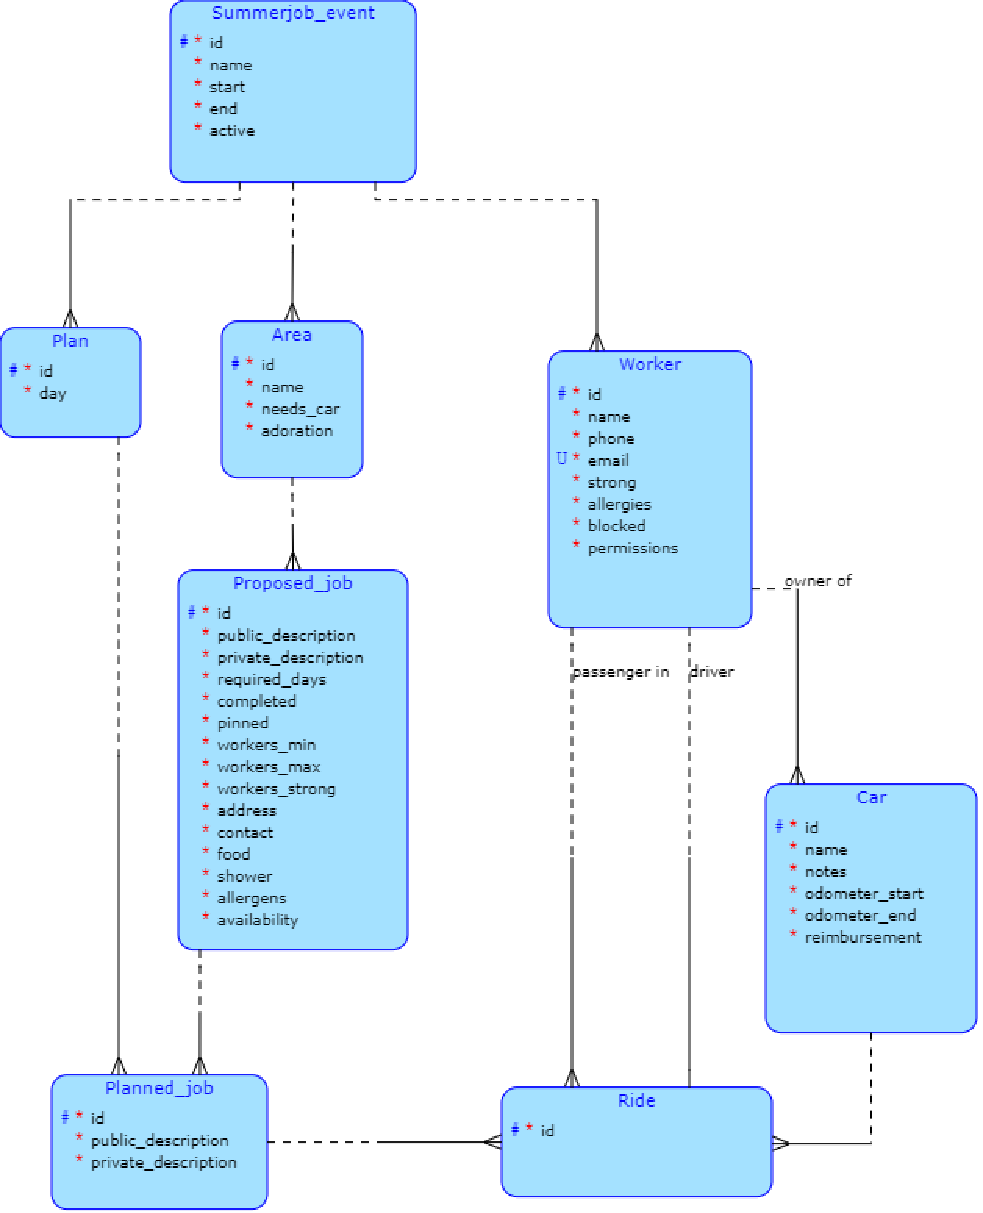
\includegraphics[width=\textwidth]{chapters/images/schema}
    \caption{Konceptuální schéma}
    \label{fig:schema}
\end{figure}


\subsection{Plánovací systém}

Automatický plánovací systém vychází z funkčního požadavku 7. Organizátoři budou mít možnost přidat do vytvořeného plánu na daný den požadované práce, které
chtějí vykonat. Tato funkce je implementována v rámci webové aplikace. Následně organizátor pomocí webové aplikace spustí proces plánování, který vygeneruje plán pro
daný den. Po dokončení se organizátorům zobrazí výsledný vygenerovaný plán.

Generování plánu zahrnuje přiřazení dostupných brigádníků k práci a přiřazení dopravy k práci, pokud je doprava vyžadována.
Plánovací systém tvoří plány podle následujících kritérií:
\begin{itemize}
    \item \textbf{Počet brigádníků na práci:} na zadanou práci musí být přiřazeno dostatečné množství brigádníků. Systém u každé práce eviduje minimální a maximální počet brigádníků, kteří mohou na místě pracovat. 
    \item \textbf{Počet silných pracantů:} na zadanou práci musí být přiřazeno dostatečné množství silných pracantů. Některé fyzicky náročné práce mohou vyžadovat přítomnost jednoho či více silných pracantů. Systém musí u každého brigádníka tento atribut evidovat.
    \item \textbf{Doprava:} pokud práce není v docházkové vzdálenosti od místa ubytování brigádníků, musí být brigádníkům přiřazena doprava. Systém musí u každé práce evidovat, zda je doprava vyžadována a u každého brigádníka evidovat, zda má k dispozici auto. Pokud je to možné, je pro práci vybrán brigádník s autem, který následně převáží ostatní brigádníky na pracoviště. Pokud jsou v autě volná místa, může řidič převážet i brigádníky z jiné práce, pokud je tato práce ve stejné oblasti jako práce řidiče (tzv. sdílená doprava).
    \item \textbf{Zodpovědný pracant:} na každou práci je zvolen jeden zodpovědný pracant, který zodpovídá za správné provedení práce a komunikuje s organizátory.
    \item \textbf{Alergie:} u práce je možné evidovat alergeny, které se na pracovišti nacházejí. Systém musí u každého brigádníka evidovat alergie a přiřazení brigádníka k práci musí být zajištěno tak, aby brigádník neměl alergii na alergeny na pracovišti.
    \item \textbf{Dostupnost pracantů:} někteří brigádníci mohou být v daný den nedostupní a nemohou se účastnit žádné práce. Systém musí u každého brigádníka evidovat, zda je v daný den dostupný. Pokud brigádník není v daný den dostupný, nesmí být přiřazen k žádné práci.
    \item \textbf{Adorace:} systém u brigádníků eviduje, zda se chtějí účastnit adorace. Adorace probíhá během dne v délce dvou hodin v některém z kostelů v okolí. Systém musí zajistit, aby brigádníci, kteří se chtějí účastnit adorace, byli přiřazeni k práci, která probíhá v blízkosti kostelu, pokud je to možné.
    \item \textbf{Zachování naplánovaných prací:} pokud jsou před začátkem automatického plánování někteří brigádníci již přiřazeni k práci, musí být jejich přiřazení zachováno. Plánovací systém nesmí odebírat přiřazené brigádníky z práce, z naplánované dopravy atd. Může však přidávat nové brigádníky k práci nebo stávajícím pracantům přiřazovat dopravu, pokud není doprava již přiřazena.
\end{itemize}

Po vygenerování může být plán upraven organizátory pomocí webové aplikace. Do vygenerovaného plánu musí být možné přidat další práce a vyžádat nové plánování.

\subsection{Grafický design}

Grafický design webové aplikace by měl rozšiřovat vizuální styl již existujících webových stránek SummerJob. Jedná se zejména o žluté barevné prvky, bezpatkový text nebo
logo SummerJob. Webová aplikace by měla být přehledná a intuitivní.

Před zahájením vývoje byl dodán základní grafický návrh aplikace, který zobrazuje vybrané prvky a stránky aplikace.
Dodaný grafický návrh neslouží jako přesný návrh vzhledu aplikace, ale jako inspirace pro vývojáře. Ukázka z dodaného návrhu je k dispozici na obrázku \ref{fig:design}.

Na základě dodaného návrhu byl vypracován detailnější grafický návrh vybraných částí aplikace, který byl před zahájením vývoje schválen organizátory.
Tento návrh byl vytvořen pomocí nástroje Bootstrap Studio, který umožňuje vytvářet grafické návrhy webových stránek pomocí interaktivního
upravování předpřipravených komponent a export návrhu do HTML a CSS \cite{bootstrap_studio}.
Ukázka je k dispozici na obrázku \ref{fig:design-detail}. Vývoj vycházel z tohoto návrhu, který byl v průběhu implementace dále upravován podle potřeb organizátorů.

\begin{figure}[ht]
    \centering
    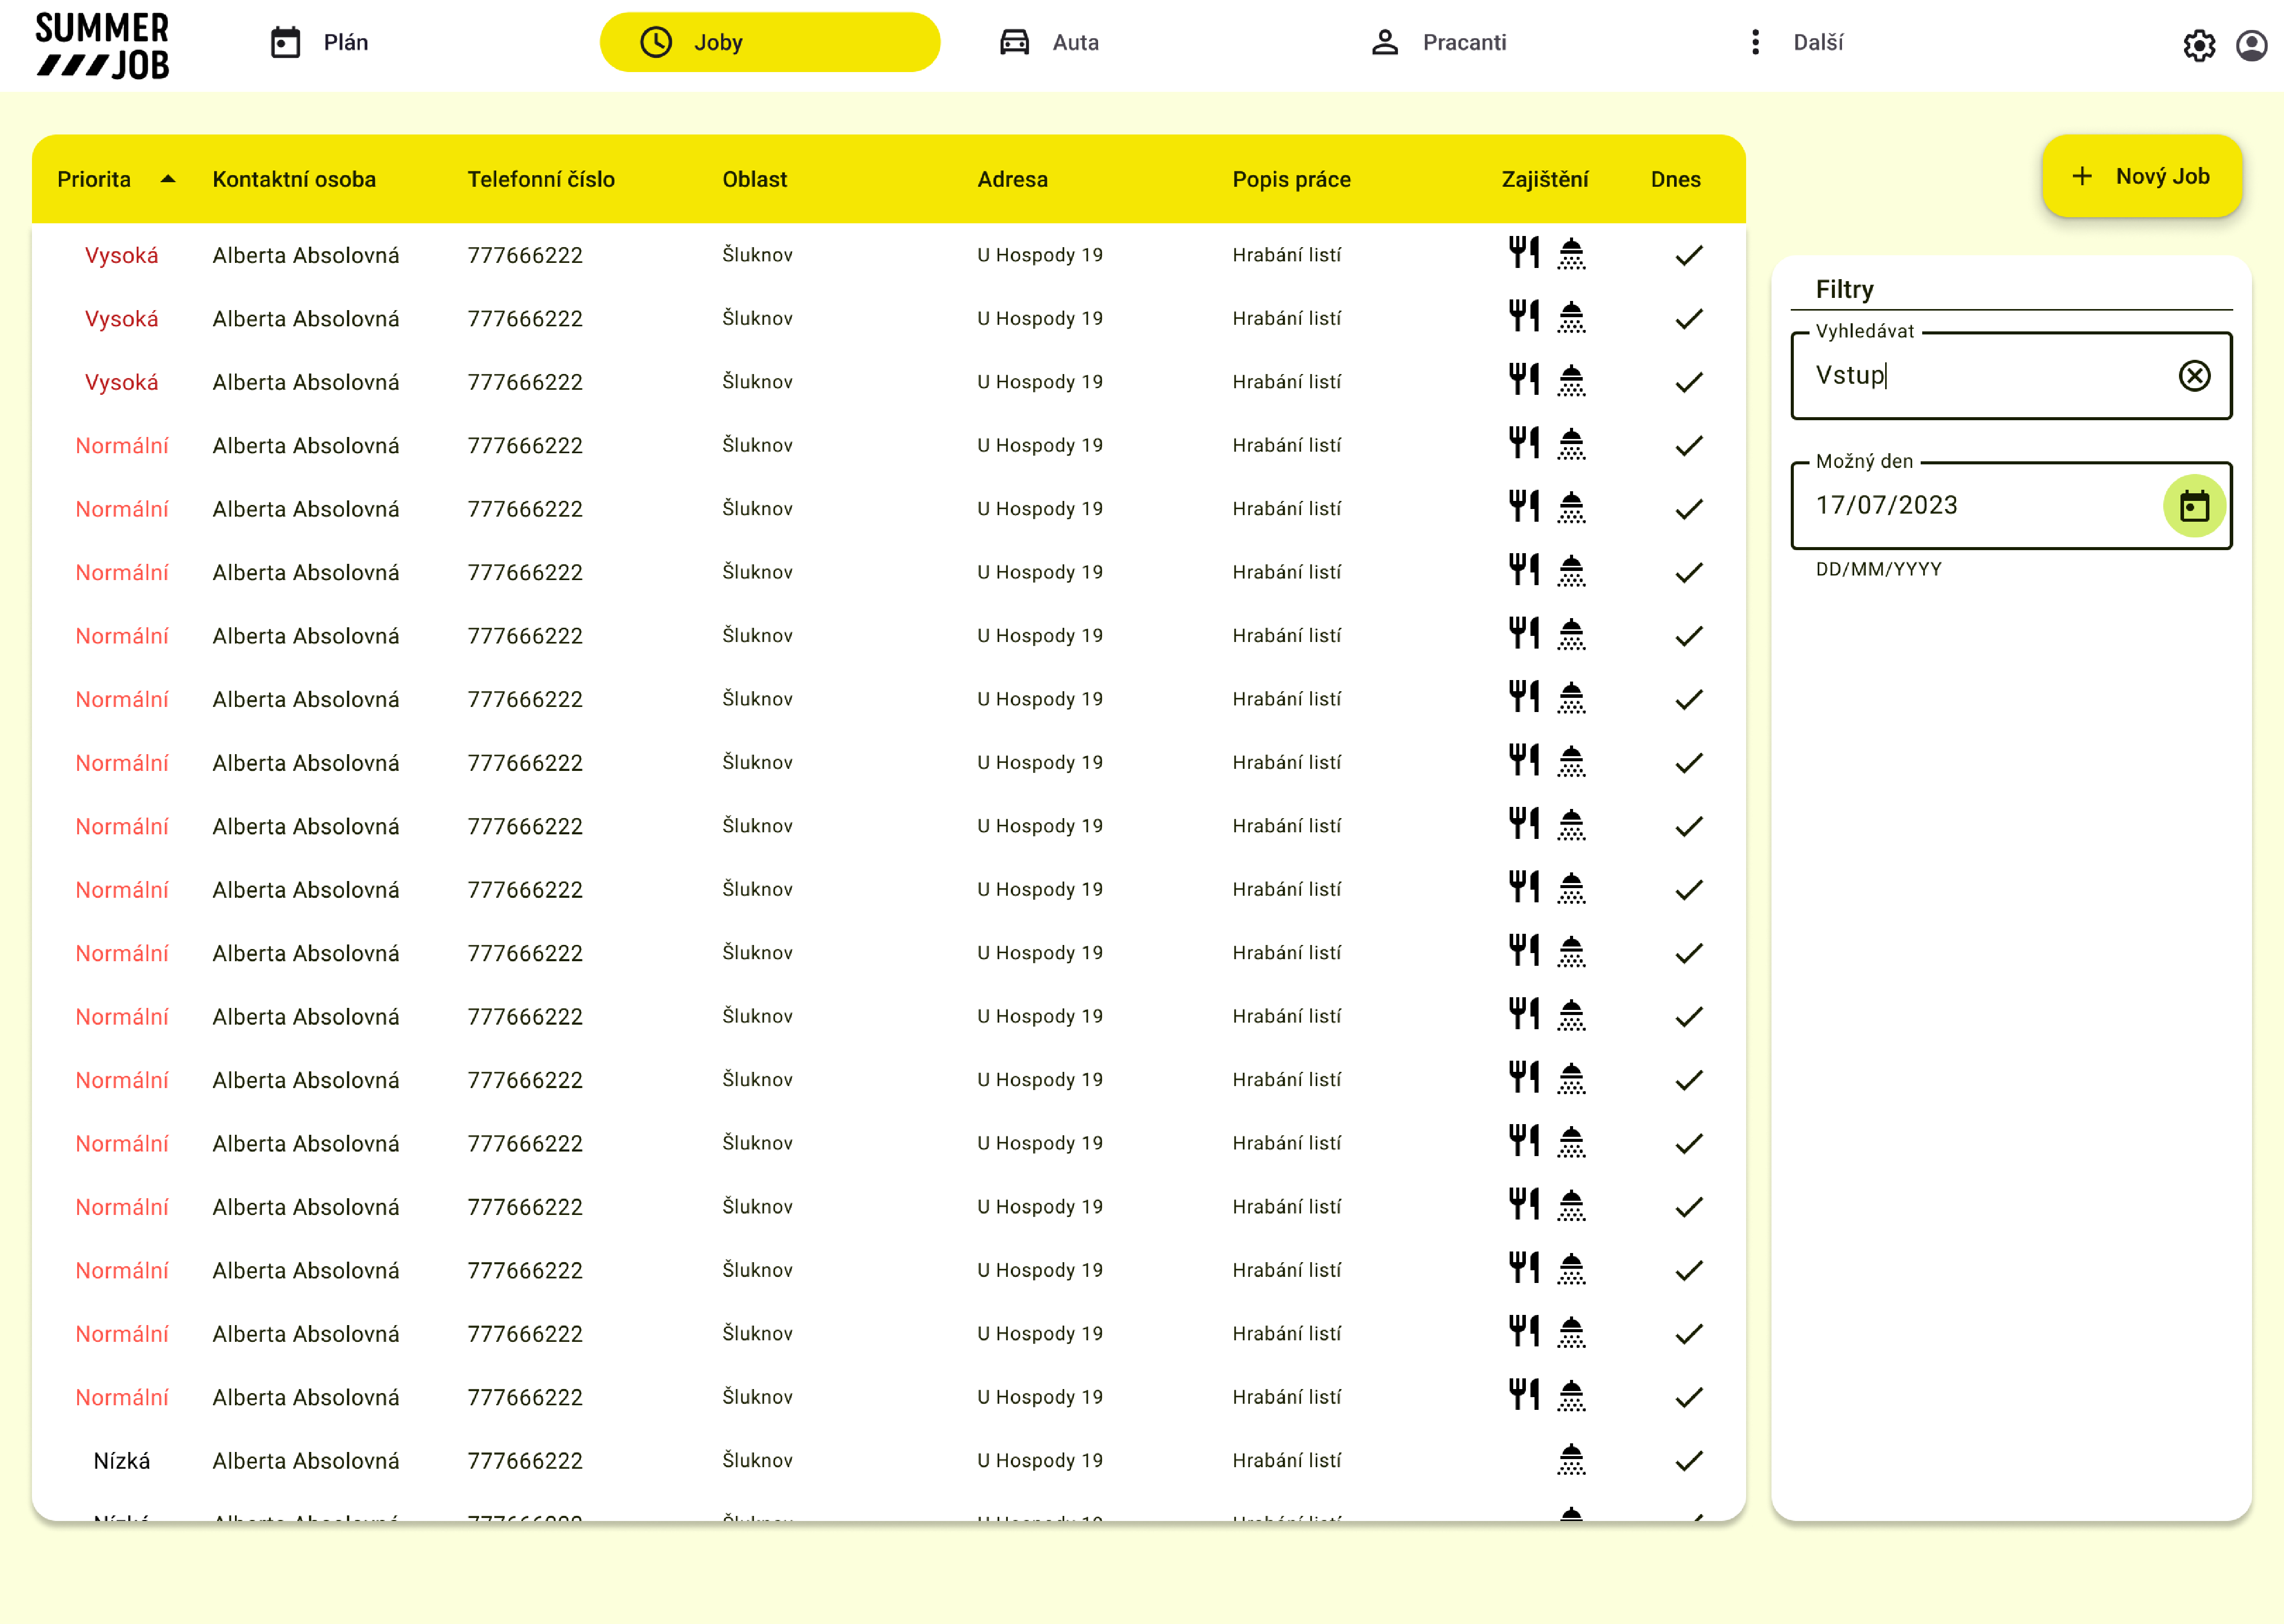
\includegraphics[width=\textwidth]{chapters/images/graficky-navrh}
    \caption{Dodaný grafický návrh webové aplikace}
    \label{fig:design}
\end{figure}

\begin{figure}[ht]
    \centering
    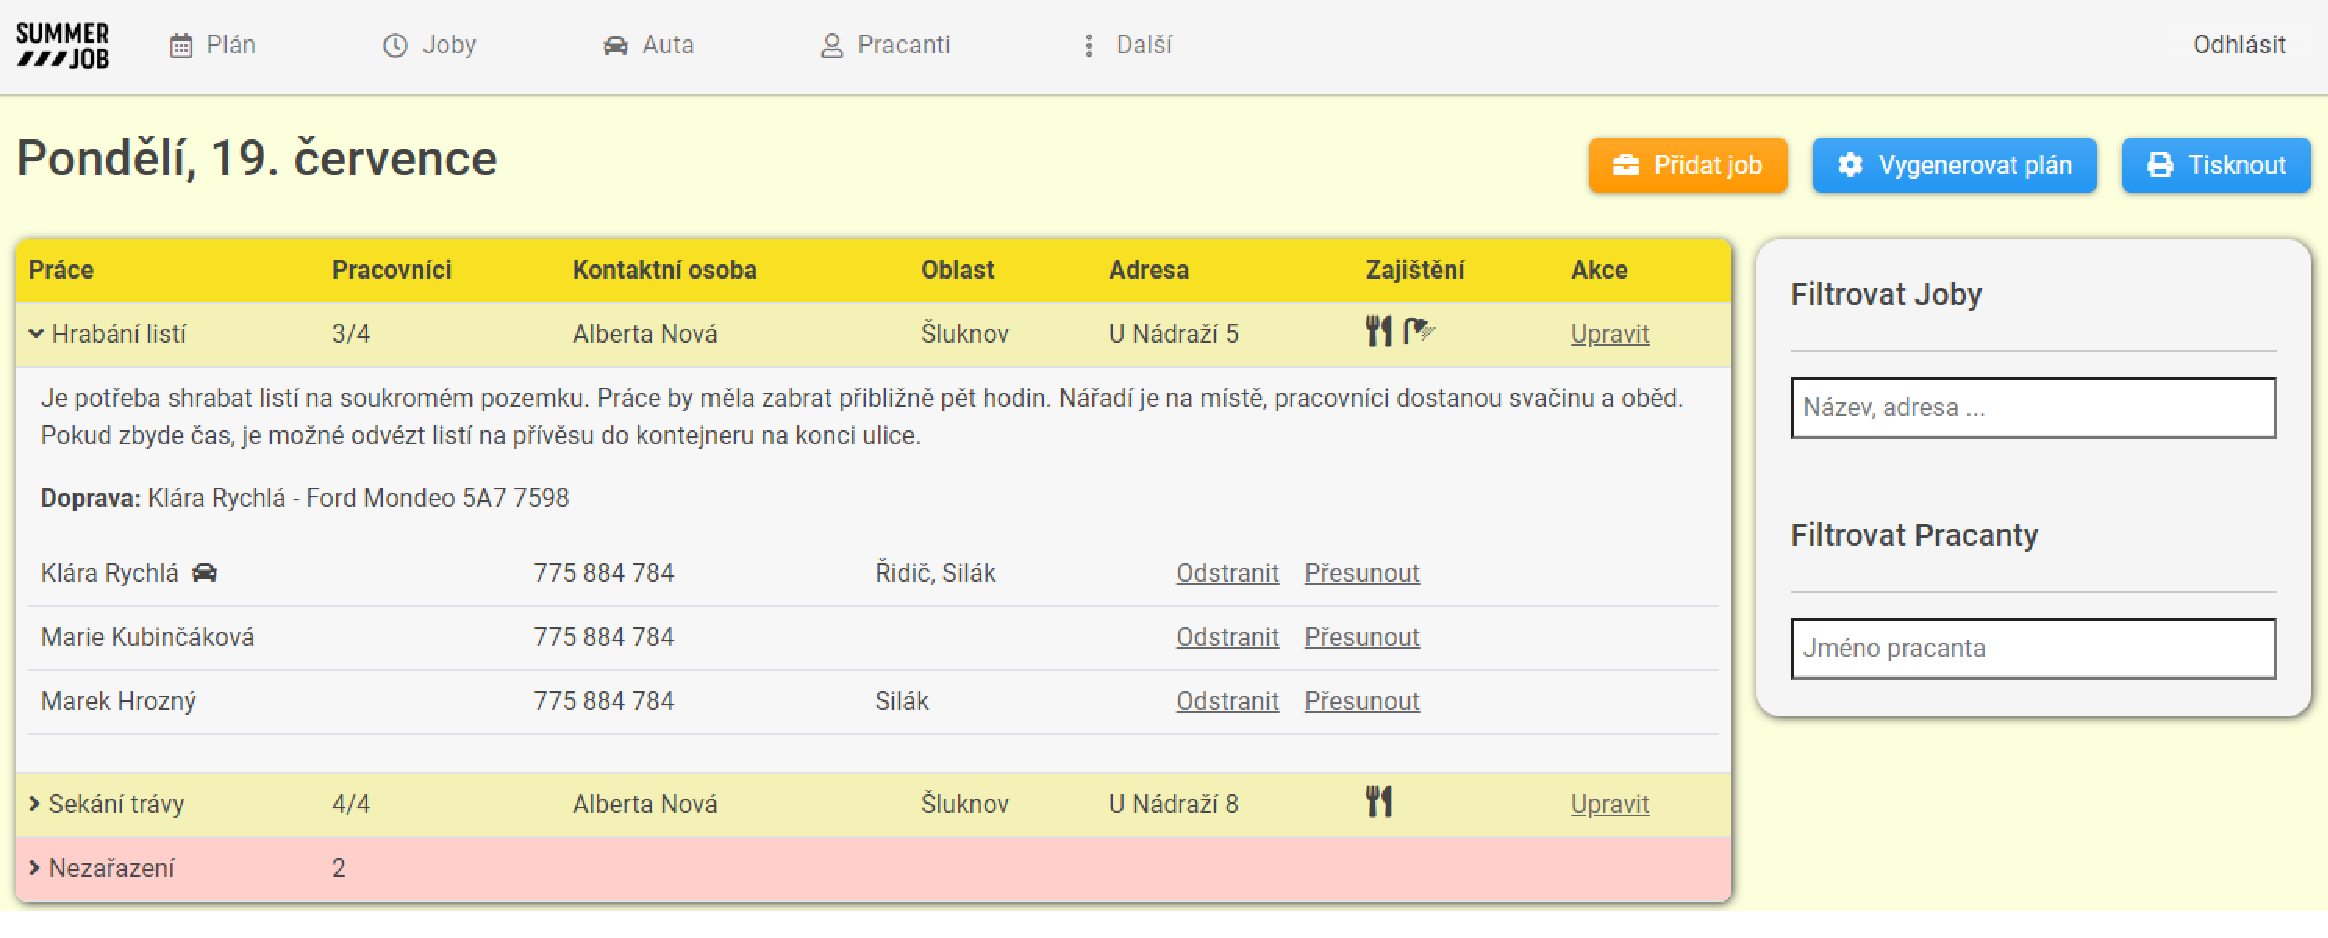
\includegraphics[width=\textwidth]{chapters/images/bootstrap-studio}
    \caption{Vytvořený grafický návrh webové aplikace}
    \label{fig:design-detail}
\end{figure}